\chapter{Supplementary Results}
\section{All tests in increasing order of mean F1-score} \label{result_all_subsets_table}

% Please add the following required packages to your document preamble:
% \usepackage{longtable}
% Note: It may be necessary to compile the document several times to get a multi-page table to line up properly
\begin{longtable}{llllll}
\hline
\multicolumn{1}{|l|}{} & \multicolumn{1}{l|}{Frequencies in test}          & \multicolumn{1}{l|}{Num} & \multicolumn{1}{l|}{Precision} & \multicolumn{1}{l|}{Recall} & \multicolumn{1}{l|}{F1\_Score} \\ \hline
\endfirsthead
%
\endhead
%
\hline
\endfoot
%
\endlastfoot
%
0                      & test\_38kHz\_18kHz\_120kHz\_200kHz                & 4                        & 0.53                           & 0.94                        & 0.67                           \\
1                      & test\_38kHz\_18kHz\_70kHz\_120kHz\_200kHz         & 5                        & 0.52                           & 0.94                        & 0.67                           \\
2                      & test\_38kHz\_18kHz\_120kHz\_200kHz\_333kHz        & 5                        & 0.53                           & 0.89                        & 0.67                           \\
3                      & test\_38kHz\_18kHz\_70kHz\_120kHz\_200kHz\_333kHz & 6                        & 0.53                           & 0.89                        & 0.66                           \\
4                      & test\_38kHz\_18kHz\_70kHz\_200kHz\_333kHz         & 5                        & 0.53                           & 0.89                        & 0.66                           \\
5                      & test\_38kHz\_18kHz\_70kHz\_200kHz                 & 4                        & 0.51                           & 0.93                        & 0.66                           \\
6                      & test\_38kHz\_18kHz\_200kHz                        & 3                        & 0.5                            & 0.93                        & 0.65                           \\
7                      & test\_38kHz\_18kHz\_200kHz\_333kHz                & 4                        & 0.51                           & 0.89                        & 0.65                           \\
8                      & test\_38kHz\_18kHz\_70kHz\_120kHz\_333kHz         & 5                        & 0.44                           & 0.86                        & 0.58                           \\
9                      & test\_38kHz\_18kHz\_120kHz\_333kHz                & 4                        & 0.44                           & 0.86                        & 0.58                           \\
10                     & test\_18kHz\_70kHz\_120kHz\_200kHz\_333kHz        & 5                        & 0.43                           & 0.89                        & 0.58                           \\
11                     & test\_18kHz\_70kHz\_200kHz\_333kHz                & 4                        & 0.42                           & 0.88                        & 0.57                           \\
12                     & test\_38kHz\_18kHz\_70kHz\_333kHz                 & 4                        & 0.42                           & 0.83                        & 0.56                           \\
13                     & test\_38kHz\_18kHz\_333kHz                        & 3                        & 0.43                           & 0.82                        & 0.56                           \\
14                     & test\_18kHz\_70kHz\_200kHz                        & 3                        & 0.39                           & 0.92                        & 0.55                           \\
15                     & test\_18kHz\_120kHz\_200kHz\_333kHz               & 4                        & 0.4                            & 0.87                        & 0.54                           \\
16                     & test\_18kHz\_70kHz\_120kHz\_200kHz                & 4                        & 0.38                           & 0.93                        & 0.54                           \\
17                     & test\_18kHz\_200kHz\_333kHz                       & 3                        & 0.4                            & 0.84                        & 0.53                           \\
18                     & test\_18kHz\_120kHz\_333kHz                       & 3                        & 0.37                           & 0.84                        & 0.51                           \\
19                     & test\_18kHz\_120kHz\_200kHz                       & 3                        & 0.36                           & 0.9                         & 0.51                           \\
20                     & test\_18kHz\_70kHz\_333kHz                        & 3                        & 0.36                           & 0.82                        & 0.5                            \\
21                     & test\_38kHz\_70kHz\_120kHz\_200kHz\_333kHz        & 5                        & 0.38                           & 0.7                         & 0.5                            \\
22                     & test\_18kHz\_70kHz\_120kHz\_333kHz                & 4                        & 0.35                           & 0.86                        & 0.49                           \\
23                     & test\_70kHz\_120kHz\_200kHz\_333kHz               & 4                        & 0.39                           & 0.66                        & 0.49                           \\
24                     & test\_38kHz\_120kHz\_200kHz\_333kHz               & 4                        & 0.37                           & 0.68                        & 0.48                           \\
25                     & test\_70kHz\_200kHz\_333kHz                       & 3                        & 0.38                           & 0.64                        & 0.47                           \\
26                     & test\_38kHz\_200kHz\_333kHz                       & 3                        & 0.37                           & 0.65                        & 0.47                           \\
27                     & test\_38kHz\_70kHz\_200kHz\_333kHz                & 4                        & 0.36                           & 0.68                        & 0.47                           \\
28                     & test\_38kHz\_70kHz\_120kHz\_200kHz                & 4                        & 0.35                           & 0.68                        & 0.46                           \\
29                     & test\_70kHz\_200kHz                               & 2                        & 0.36                           & 0.64                        & 0.46                           \\
30                     & test\_18kHz\_333kHz                               & 2                        & 0.34                           & 0.73                        & 0.46                           \\
31                     & test\_70kHz\_120kHz\_200kHz                       & 3                        & 0.35                           & 0.64                        & 0.45                           \\
32                     & test\_38kHz\_70kHz\_200kHz                        & 3                        & 0.34                           & 0.68                        & 0.45                           \\
33                     & test\_18kHz\_200kHz                               & 2                        & 0.3                            & 0.84                        & 0.45                           \\
34                     & test\_38kHz\_120kHz\_200kHz                       & 3                        & 0.33                           & 0.68                        & 0.44                           \\
35                     & test\_38kHz\_18kHz\_70kHz\_120kHz                 & 4                        & 0.3                            & 0.88                        & 0.44                           \\
36                     & test\_38kHz\_200kHz                               & 2                        & 0.32                           & 0.67                        & 0.44                           \\
37                     & test\_38kHz\_333kHz                               & 2                        & 0.35                           & 0.54                        & 0.43                           \\
38                     & test\_18kHz\_70kHz\_120kHz                        & 3                        & 0.28                           & 0.86                        & 0.42                           \\
39                     & test\_38kHz\_70kHz\_120kHz\_333kHz                & 4                        & 0.31                           & 0.63                        & 0.42                           \\
40                     & test\_120kHz\_200kHz\_333kHz                      & 3                        & 0.34                           & 0.53                        & 0.41                           \\
41                     & test\_38kHz\_70kHz\_333kHz                        & 3                        & 0.31                           & 0.62                        & 0.41                           \\
42                     & test\_38kHz\_18kHz\_120kHz                        & 3                        & 0.27                           & 0.88                        & 0.41                           \\
43                     & test\_70kHz\_120kHz\_333kHz                       & 3                        & 0.32                           & 0.56                        & 0.4                            \\
44                     & test\_70kHz\_120kHz                               & 2                        & 0.3                            & 0.62                        & 0.4                            \\
45                     & test\_38kHz\_120kHz\_333kHz                       & 3                        & 0.3                            & 0.57                        & 0.39                           \\
46                     & test\_70kHz\_333kHz                               & 2                        & 0.32                           & 0.48                        & 0.38                           \\
47                     & test\_200kHz\_333kHz                              & 2                        & 0.31                           & 0.48                        & 0.37                           \\
48                     & test\_18kHz\_120kHz                               & 2                        & 0.23                           & 0.84                        & 0.37                           \\
49                     & test\_120kHz\_200kHz                              & 2                        & 0.28                           & 0.51                        & 0.36                           \\
50                     & test\_38kHz\_70kHz\_120kHz                        & 3                        & 0.25                           & 0.64                        & 0.36                           \\
51                     & test\_120kHz\_333kHz                              & 2                        & 0.29                           & 0.44                        & 0.35                           \\
52                     & test\_18kHz\_70kHz                                & 2                        & 0.23                           & 0.78                        & 0.35                           \\
53                     & test\_200kHz                                      & 1                        & 0.28                           & 0.47                        & 0.34                           \\
54                     & test\_38kHz\_18kHz\_70kHz                         & 3                        & 0.22                           & 0.81                        & 0.34                           \\
55                     & test\_38kHz\_18kHz                                & 2                        & 0.22                           & 0.76                        & 0.34                           \\
56                     & test\_38kHz\_120kHz                               & 2                        & 0.23                           & 0.64                        & 0.34                           \\
57                     & test\_70kHz                                       & 1                        & 0.22                           & 0.51                        & 0.3                            \\
58                     & test\_120kHz                                      & 1                        & 0.21                           & 0.48                        & 0.29                           \\
59                     & test\_38kHz\_70kHz                                & 2                        & 0.19                           & 0.57                        & 0.28                           \\
60                     & test\_18kHz                                       & 1                        & 0.19                           & 0.49                        & 0.27                           \\
61                     & test\_38kHz                                       & 1                        & 0.18                           & 0.5                         & 0.26                           \\
62                     & test\_333kHz                                      & 1                        & 0.22                           & 0.34                        & 0.25                           \\ \hline
\end{longtable}


\section{Tests per subset size in increasing order of mean F1-score} \label{test_per_freq_f1_appendix}

% Please add the following required packages to your document preamble:
% \usepackage{longtable}
% Note: It may be necessary to compile the document several times to get a multi-page table to line up properly
\begin{longtable}{lllll}
\hline
\multicolumn{1}{|l|}{} & \multicolumn{1}{l|}{Frequencies in test(1)} & \multicolumn{1}{l|}{Precision} & \multicolumn{1}{l|}{Recall} & \multicolumn{1}{l|}{F1\_Score} \\ \hline
\endfirsthead
%
\endhead
%
\hline
\endfoot
%
\endlastfoot
%
0                      & test\_200kHz                                & 0.28                           & 0.47                        & 0.34                           \\
1                      & test\_70kHz                                 & 0.22                           & 0.51                        & 0.3                            \\
2                      & test\_120kHz                                & 0.21                           & 0.48                        & 0.29                           \\
3                      & test\_18kHz                                 & 0.19                           & 0.49                        & 0.27                           \\
4                      & test\_38kHz                                 & 0.18                           & 0.5                         & 0.26                           \\
5                      & test\_333kHz                                & 0.22                           & 0.34                        & 0.25                           \\ \hline
\end{longtable}
% Please add the following required packages to your document preamble:
% \usepackage{longtable}
% Note: It may be necessary to compile the document several times to get a multi-page table to line up properly
\begin{longtable}{lllll}
\hline
\multicolumn{1}{|l|}{} & \multicolumn{1}{l|}{Frequencies in test(2)} & \multicolumn{1}{l|}{Precision} & \multicolumn{1}{l|}{Recall} & \multicolumn{1}{l|}{F1\_Score} \\ \hline
\endfirsthead
%
\endhead
%
\hline
\endfoot
%
\endlastfoot
%
0                      & test\_70kHz\_200kHz                         & 0.36                           & 0.64                        & 0.46                           \\
1                      & test\_18kHz\_333kHz                         & 0.34                           & 0.73                        & 0.46                           \\
2                      & test\_18kHz\_200kHz                         & 0.3                            & 0.84                        & 0.45                           \\
3                      & test\_38kHz\_200kHz                         & 0.32                           & 0.67                        & 0.44                           \\
4                      & test\_38kHz\_333kHz                         & 0.35                           & 0.54                        & 0.43                           \\
5                      & test\_70kHz\_120kHz                         & 0.3                            & 0.62                        & 0.4                            \\
6                      & test\_70kHz\_333kHz                         & 0.32                           & 0.48                        & 0.38                           \\
7                      & test\_200kHz\_333kHz                        & 0.31                           & 0.48                        & 0.37                           \\
8                      & test\_18kHz\_120kHz                         & 0.23                           & 0.84                        & 0.37                           \\
9                      & test\_120kHz\_200kHz                        & 0.28                           & 0.51                        & 0.36                           \\
10                     & test\_120kHz\_333kHz                        & 0.29                           & 0.44                        & 0.35                           \\
11                     & test\_18kHz\_70kHz                          & 0.23                           & 0.78                        & 0.35                           \\
12                     & test\_38kHz\_18kHz                          & 0.22                           & 0.76                        & 0.34                           \\
13                     & test\_38kHz\_120kHz                         & 0.23                           & 0.64                        & 0.34                           \\
14                     & test\_38kHz\_70kHz                          & 0.19                           & 0.57                        & 0.28                           \\ \hline
\end{longtable}

% Please add the following required packages to your document preamble:
% \usepackage{longtable}
% Note: It may be necessary to compile the document several times to get a multi-page table to line up properly
\begin{longtable}{lllll}
\hline
\multicolumn{1}{|l|}{} & \multicolumn{1}{l|}{Frequencies in test(3)} & \multicolumn{1}{l|}{Precision} & \multicolumn{1}{l|}{Recall} & \multicolumn{1}{l|}{F1\_Score} \\ \hline
\endfirsthead
%
\endhead
%
\hline
\endfoot
%
\endlastfoot
%
0                      & test\_38kHz\_18kHz\_200kHz                  & 0.5                            & 0.93                        & 0.65                           \\
1                      & test\_38kHz\_18kHz\_333kHz                  & 0.43                           & 0.82                        & 0.56                           \\
2                      & test\_18kHz\_70kHz\_200kHz                  & 0.39                           & 0.92                        & 0.55                           \\
3                      & test\_18kHz\_200kHz\_333kHz                 & 0.4                            & 0.84                        & 0.53                           \\
4                      & test\_18kHz\_120kHz\_333kHz                 & 0.37                           & 0.84                        & 0.51                           \\
5                      & test\_18kHz\_120kHz\_200kHz                 & 0.36                           & 0.9                         & 0.51                           \\
6                      & test\_18kHz\_70kHz\_333kHz                  & 0.36                           & 0.82                        & 0.5                            \\
7                      & test\_70kHz\_200kHz\_333kHz                 & 0.38                           & 0.64                        & 0.47                           \\
8                      & test\_38kHz\_200kHz\_333kHz                 & 0.37                           & 0.65                        & 0.47                           \\
9                      & test\_70kHz\_120kHz\_200kHz                 & 0.35                           & 0.64                        & 0.45                           \\
10                     & test\_38kHz\_70kHz\_200kHz                  & 0.34                           & 0.68                        & 0.45                           \\
11                     & test\_38kHz\_120kHz\_200kHz                 & 0.33                           & 0.68                        & 0.44                           \\
12                     & test\_18kHz\_70kHz\_120kHz                  & 0.28                           & 0.86                        & 0.42                           \\
13                     & test\_120kHz\_200kHz\_333kHz                & 0.34                           & 0.53                        & 0.41                           \\
14                     & test\_38kHz\_70kHz\_333kHz                  & 0.31                           & 0.62                        & 0.41                           \\
15                     & test\_38kHz\_18kHz\_120kHz                  & 0.27                           & 0.88                        & 0.41                           \\
16                     & test\_70kHz\_120kHz\_333kHz                 & 0.32                           & 0.56                        & 0.4                            \\
17                     & test\_38kHz\_120kHz\_333kHz                 & 0.3                            & 0.57                        & 0.39                           \\
18                     & test\_38kHz\_70kHz\_120kHz                  & 0.25                           & 0.64                        & 0.36                           \\
19                     & test\_38kHz\_18kHz\_70kHz                   & 0.22                           & 0.81                        & 0.34                           \\ \hline
\end{longtable}

% Please add the following required packages to your document preamble:
% \usepackage{longtable}
% Note: It may be necessary to compile the document several times to get a multi-page table to line up properly
\begin{longtable}{lllll}
\hline
\multicolumn{1}{|l|}{} & \multicolumn{1}{l|}{Frequencies in test(4)} & \multicolumn{1}{l|}{Precision} & \multicolumn{1}{l|}{Recall} & \multicolumn{1}{l|}{F1\_Score} \\ \hline
\endfirsthead
%
\endhead
%
\hline
\endfoot
%
\endlastfoot
%
0                      & test\_38kHz\_18kHz\_120kHz\_200kHz          & 0.53                           & 0.94                        & 0.67                           \\
1                      & test\_38kHz\_18kHz\_70kHz\_200kHz           & 0.51                           & 0.93                        & 0.66                           \\
2                      & test\_38kHz\_18kHz\_200kHz\_333kHz          & 0.51                           & 0.89                        & 0.65                           \\
3                      & test\_38kHz\_18kHz\_120kHz\_333kHz          & 0.44                           & 0.86                        & 0.58                           \\
4                      & test\_18kHz\_70kHz\_200kHz\_333kHz          & 0.42                           & 0.88                        & 0.57                           \\
5                      & test\_38kHz\_18kHz\_70kHz\_333kHz           & 0.42                           & 0.83                        & 0.56                           \\
6                      & test\_18kHz\_120kHz\_200kHz\_333kHz         & 0.4                            & 0.87                        & 0.54                           \\
7                      & test\_18kHz\_70kHz\_120kHz\_200kHz          & 0.38                           & 0.93                        & 0.54                           \\
8                      & test\_18kHz\_70kHz\_120kHz\_333kHz          & 0.35                           & 0.86                        & 0.49                           \\
9                      & test\_70kHz\_120kHz\_200kHz\_333kHz         & 0.39                           & 0.66                        & 0.49                           \\
10                     & test\_38kHz\_120kHz\_200kHz\_333kHz         & 0.37                           & 0.68                        & 0.48                           \\
11                     & test\_38kHz\_70kHz\_200kHz\_333kHz          & 0.36                           & 0.68                        & 0.47                           \\
12                     & test\_38kHz\_70kHz\_120kHz\_200kHz          & 0.35                           & 0.68                        & 0.46                           \\
13                     & test\_38kHz\_18kHz\_70kHz\_120kHz           & 0.3                            & 0.88                        & 0.44                           \\
14                     & test\_38kHz\_70kHz\_120kHz\_333kHz          & 0.31                           & 0.63                        & 0.42                           \\ \hline
\end{longtable}

% Please add the following required packages to your document preamble:
% \usepackage{longtable}
% Note: It may be necessary to compile the document several times to get a multi-page table to line up properly
\begin{longtable}{lllll}
\hline
\multicolumn{1}{|l|}{} & \multicolumn{1}{l|}{Frequencies in test(5)} & \multicolumn{1}{l|}{Precision} & \multicolumn{1}{l|}{Recall} & \multicolumn{1}{l|}{F1\_Score} \\ \hline
\endfirsthead
%
\endhead
%
\hline
\endfoot
%
\endlastfoot
%
0                      & test\_38kHz\_18kHz\_70kHz\_120kHz\_200kHz   & 0.52                           & 0.94                        & 0.67                           \\
1                      & test\_38kHz\_18kHz\_120kHz\_200kHz\_333kHz  & 0.53                           & 0.89                        & 0.67                           \\
2                      & test\_38kHz\_18kHz\_70kHz\_200kHz\_333kHz   & 0.53                           & 0.89                        & 0.66                           \\
3                      & test\_38kHz\_18kHz\_70kHz\_120kHz\_333kHz   & 0.44                           & 0.86                        & 0.58                           \\
4                      & test\_18kHz\_70kHz\_120kHz\_200kHz\_333kHz  & 0.43                           & 0.89                        & 0.58                           \\
5                      & test\_38kHz\_70kHz\_120kHz\_200kHz\_333kHz  & 0.38                           & 0.7                         & 0.5                            \\ \hline
\end{longtable}

% Please add the following required packages to your document preamble:
% \usepackage{longtable}
% Note: It may be necessary to compile the document several times to get a multi-page table to line up properly
\begin{longtable}{lllll}
\hline
\multicolumn{1}{|l|}{} & \multicolumn{1}{l|}{Frequencies in test(6)}       & \multicolumn{1}{l|}{Precision} & \multicolumn{1}{l|}{Recall} & \multicolumn{1}{l|}{F1\_Score} \\ \hline
\endfirsthead
%
\endhead
%
0                      & test\_38kHz\_18kHz\_70kHz\_120kHz\_200kHz\_333kHz & 0.53                           & 0.89                        & 0.66                           \\ \hline
\end{longtable}



\section{Training examples} \label{examples training}
    This section includes more visualizations from the monitoring during training. At a subset size of one, we provide three illustrations from different tests, while only one plot from a common test is shown for increasing subsets up to, and including, five frequencies.
    
    \subsection{Subset size 1}
        \begin{figure}[H]
             %scale=0.4,

            \hspace*{-3.2cm}
            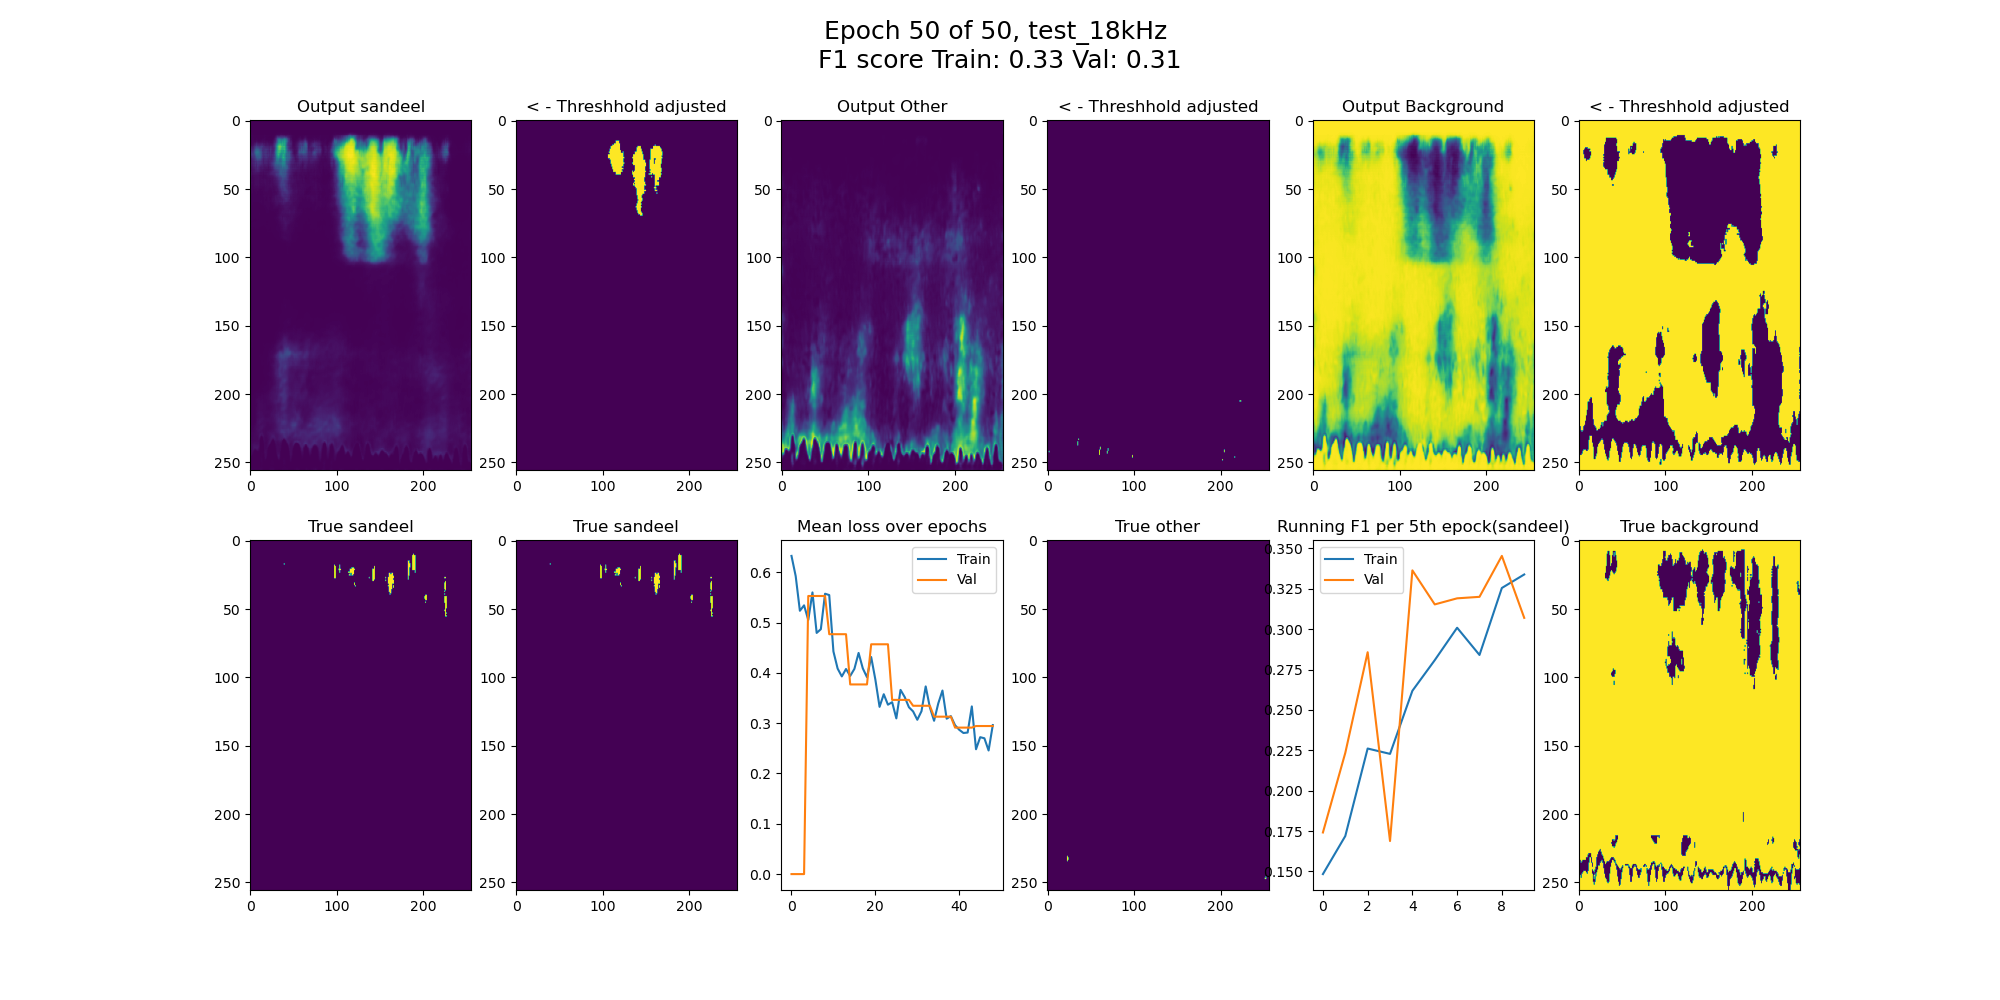
\includegraphics[scale=0.45]{figures/epoch_50_test_18kHz.png}

          	\medskip 
        \end{figure}
    \clearpage
        \begin{figure}[H]
             %scale=0.4,

            \hspace*{-3.2cm}
            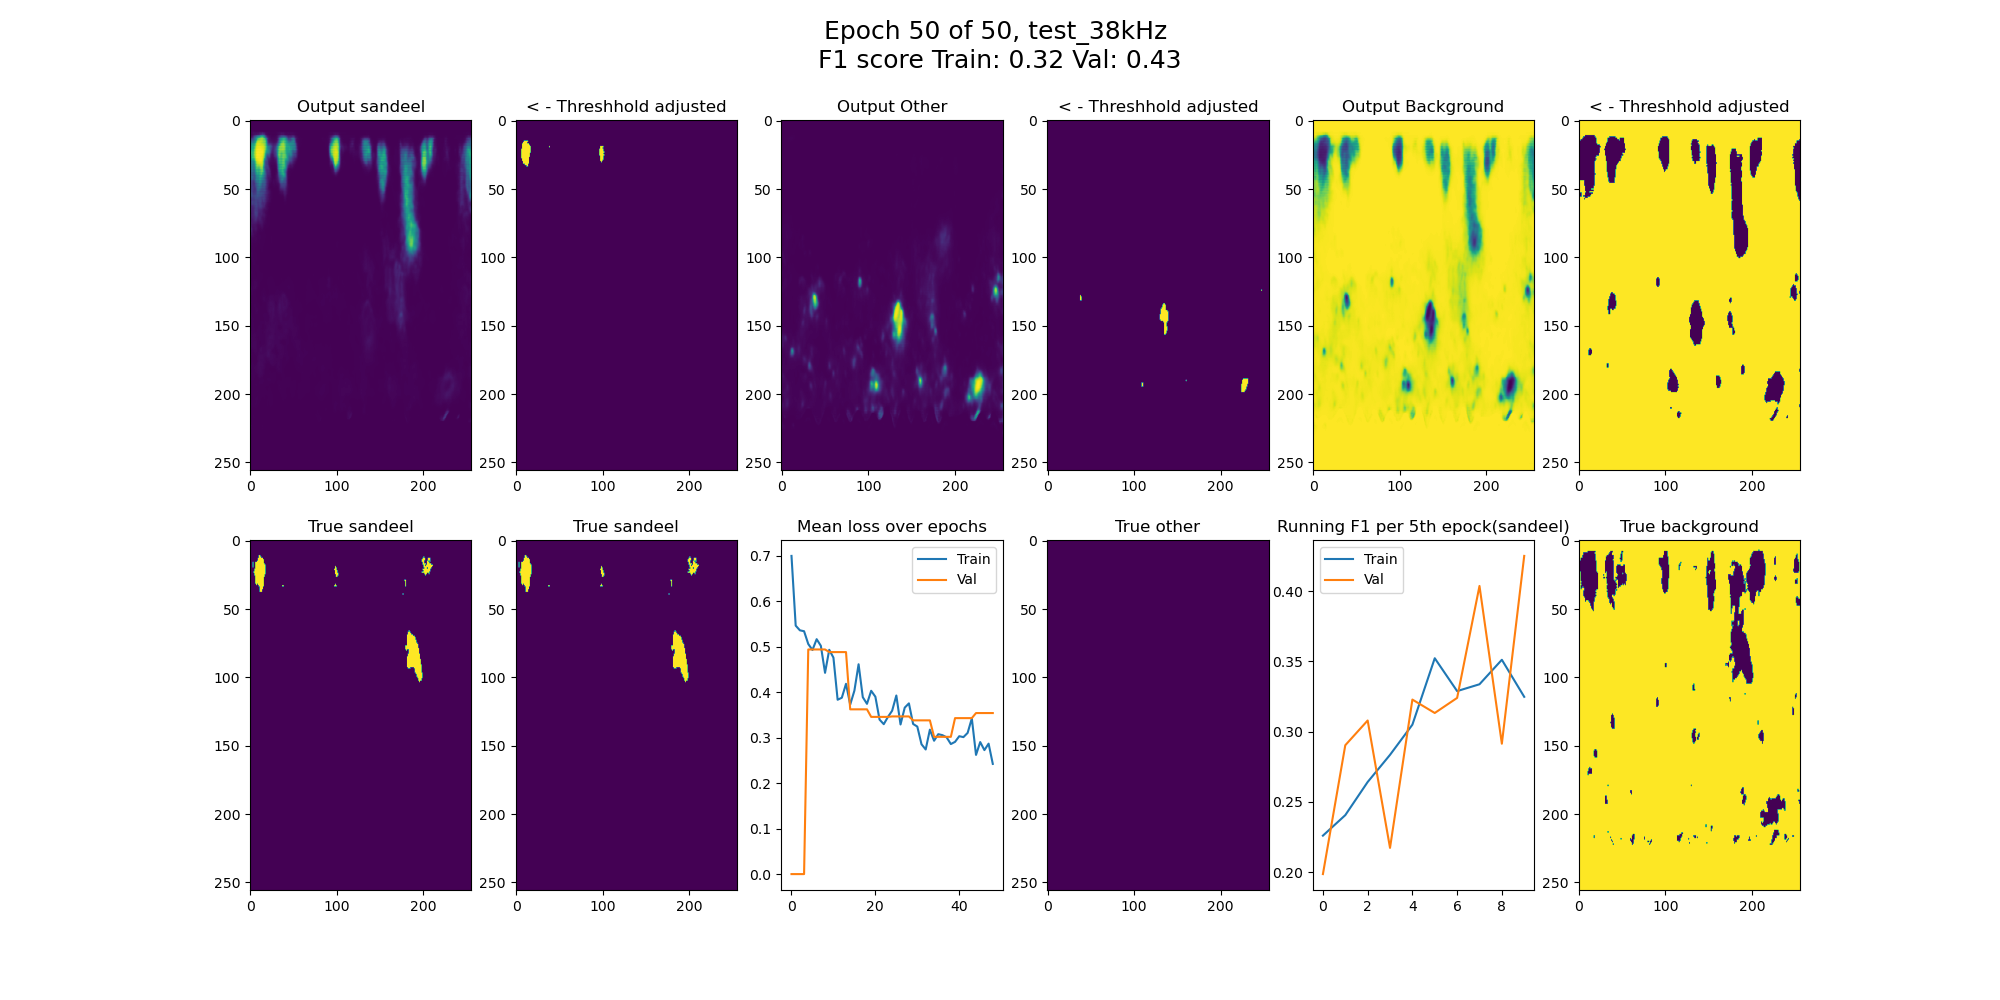
\includegraphics[scale=0.45]{figures/epoch_50_test_38kHz.png}

          	\medskip 
        \end{figure}
    \clearpage
        \begin{figure}[H]
             %scale=0.4,

            \hspace*{-3.2cm}
            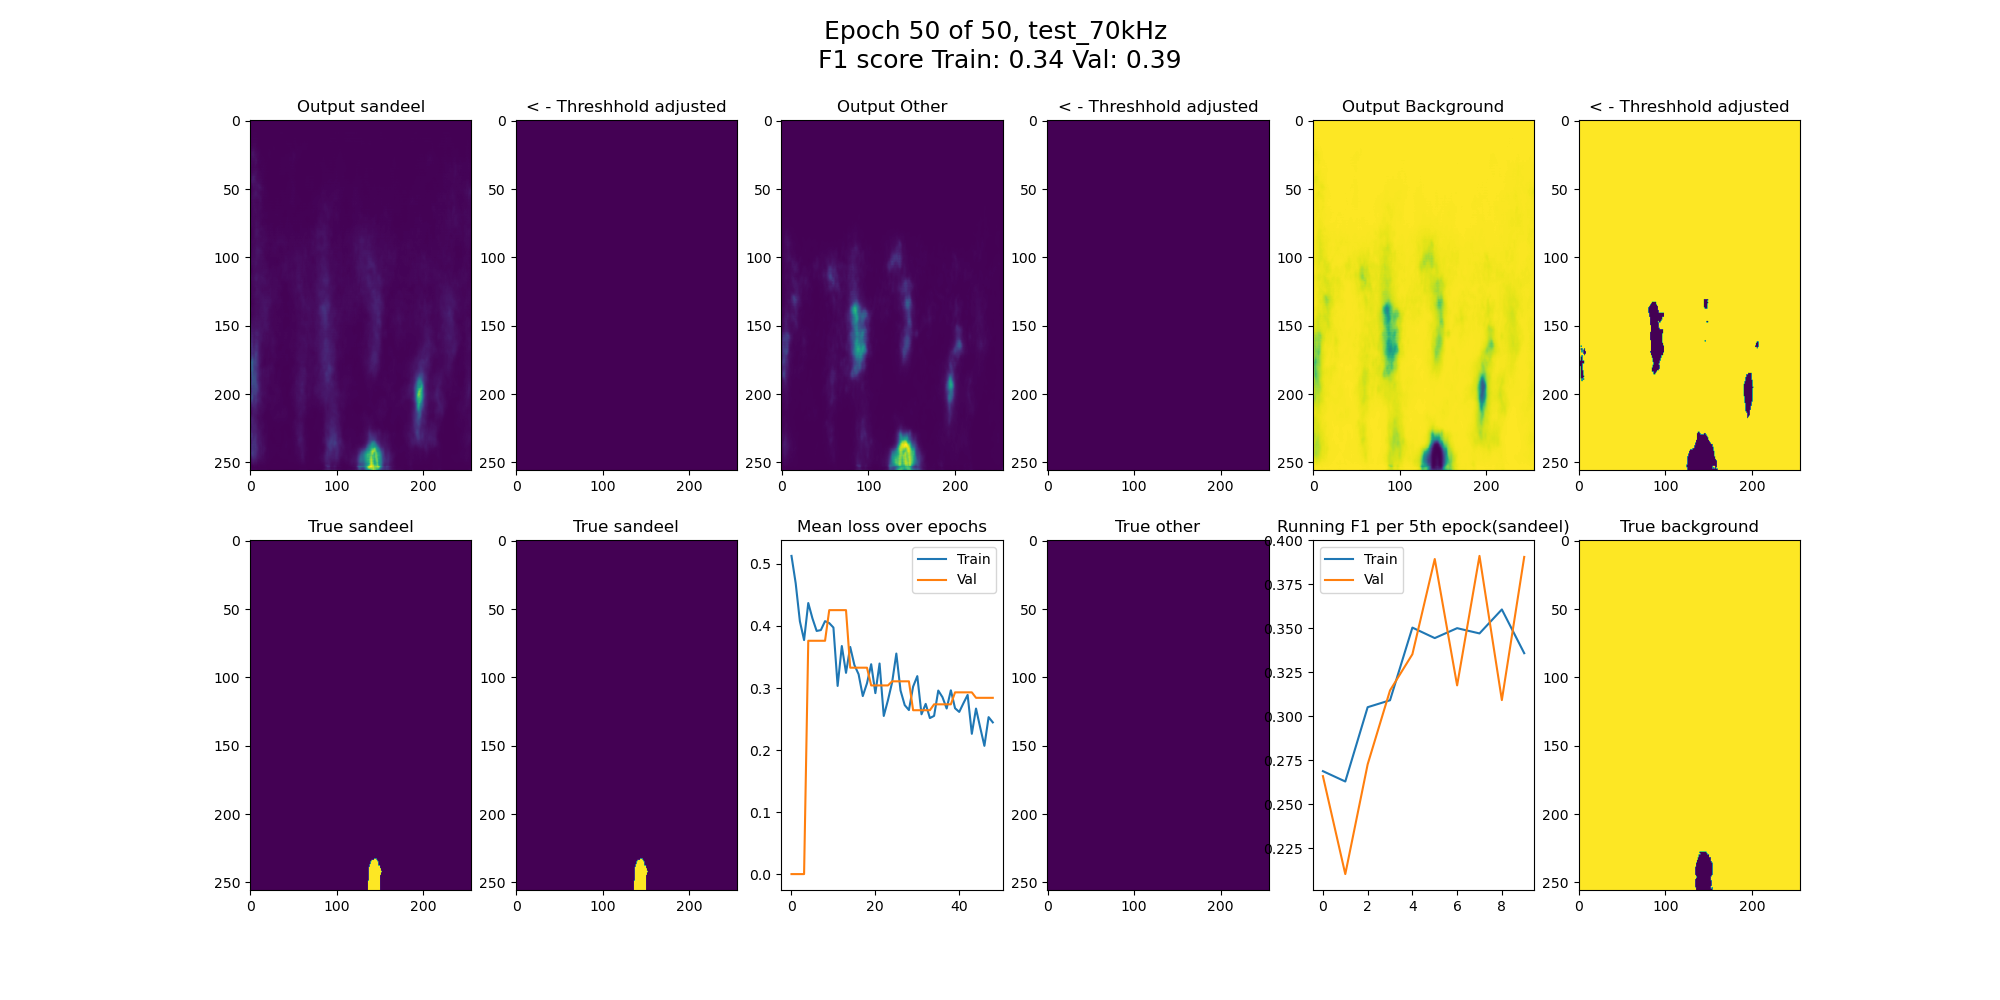
\includegraphics[scale=0.45]{figures/epoch_50_test_70kHz.png}

          	\medskip 
        \end{figure}
    \clearpage
    \subsection{Subset size 2}
        \begin{figure}[H]
             %scale=0.4,

            \hspace*{-3.2cm}
            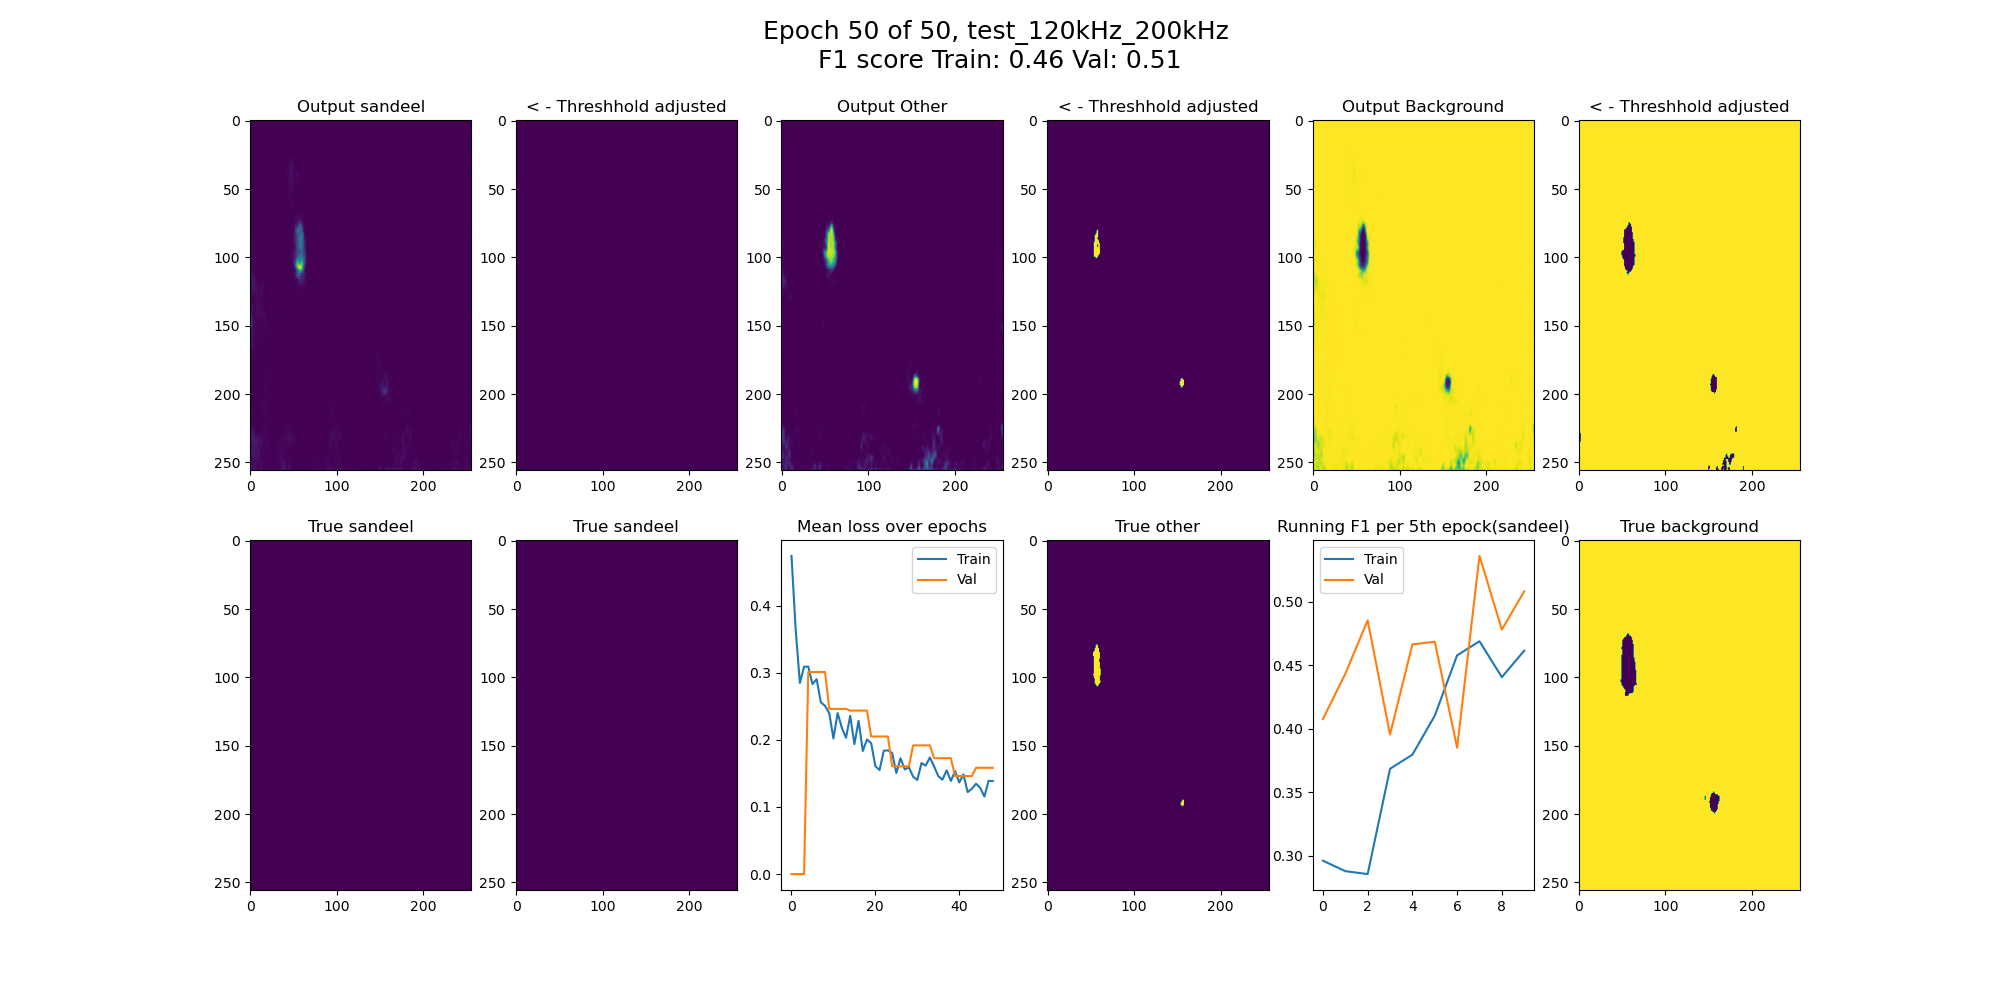
\includegraphics[scale=0.45]{figures/epoch_50_test_120kHz_200kHz.png}

          	\medskip 
        \end{figure}
    \clearpage
    \subsection{Subset size 3}
        \begin{figure}[H]
             %scale=0.4,

            \hspace*{-3.2cm}
            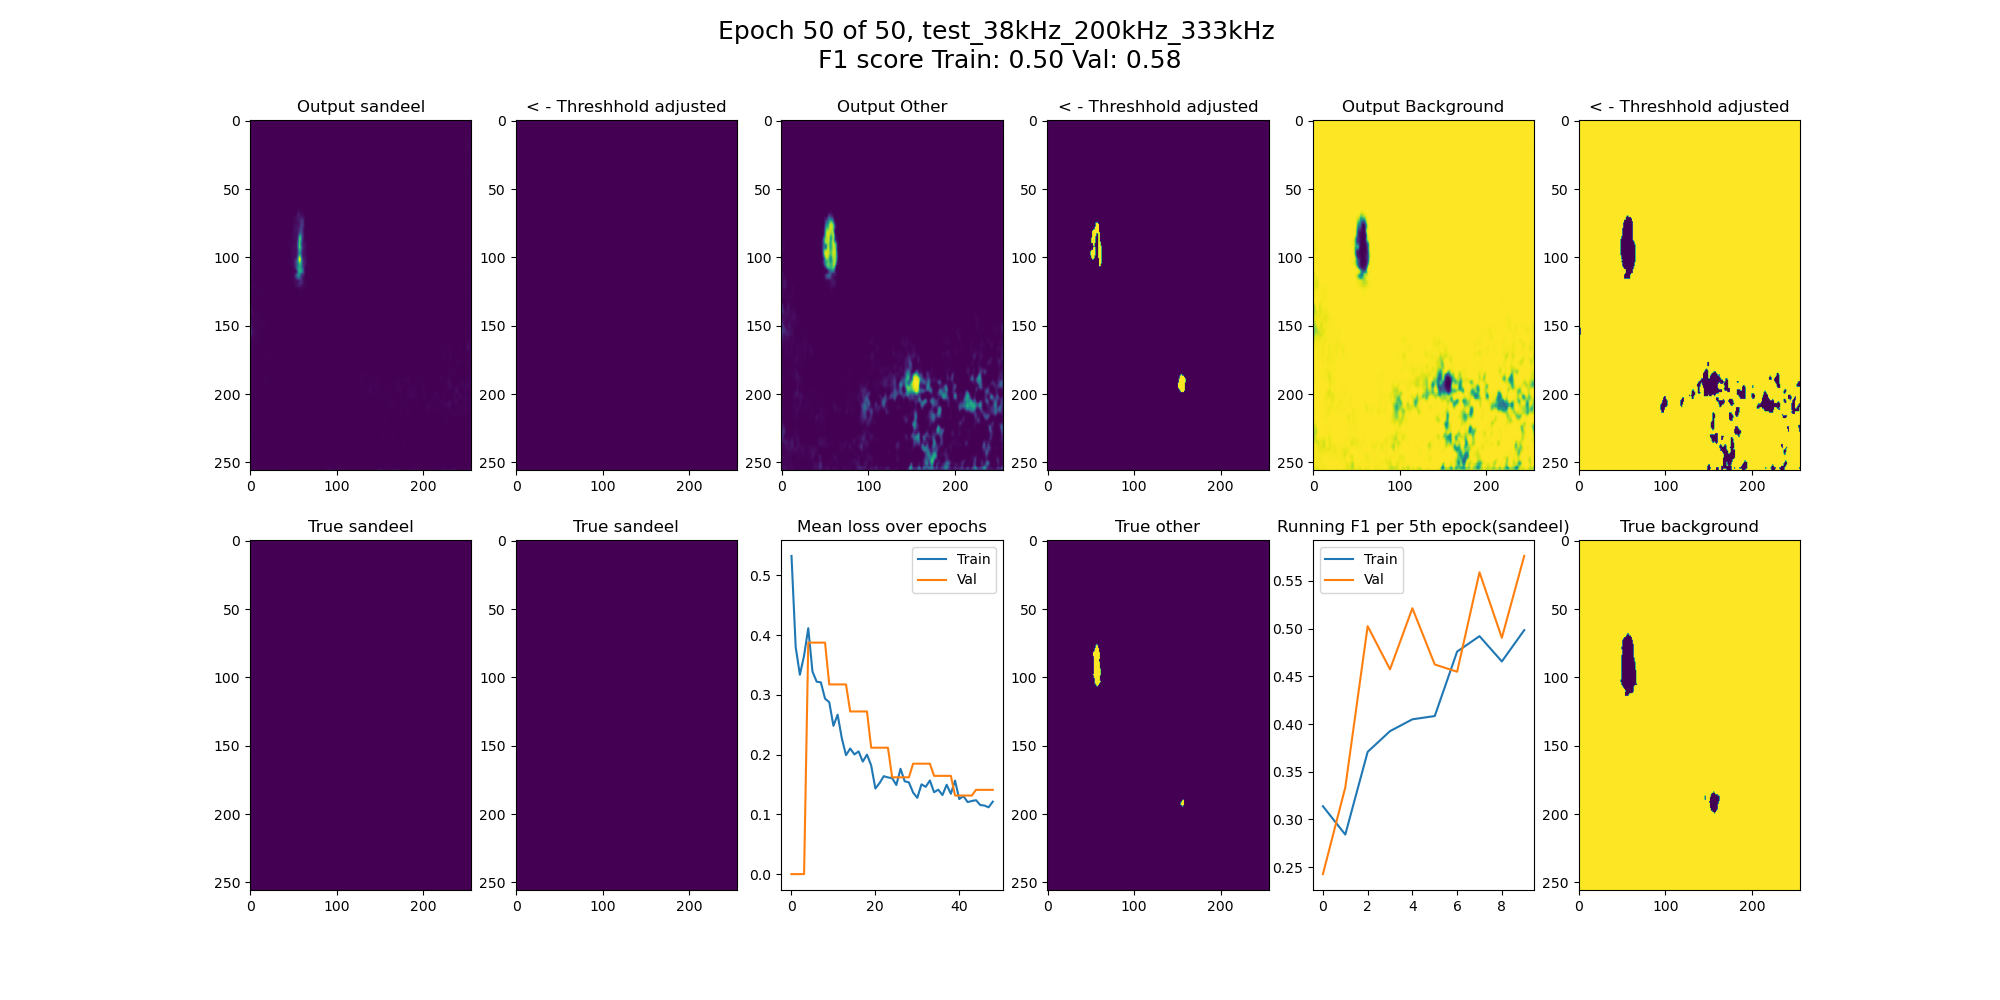
\includegraphics[scale=0.45]{figures/epoch_50_test_38kHz_200kHz_333kHz.png}

          	\medskip 
        \end{figure}
    \clearpage
    \subsection{Subset size 4}
        \begin{figure}[H]
             %scale=0.4,

            \hspace*{-3.2cm}
            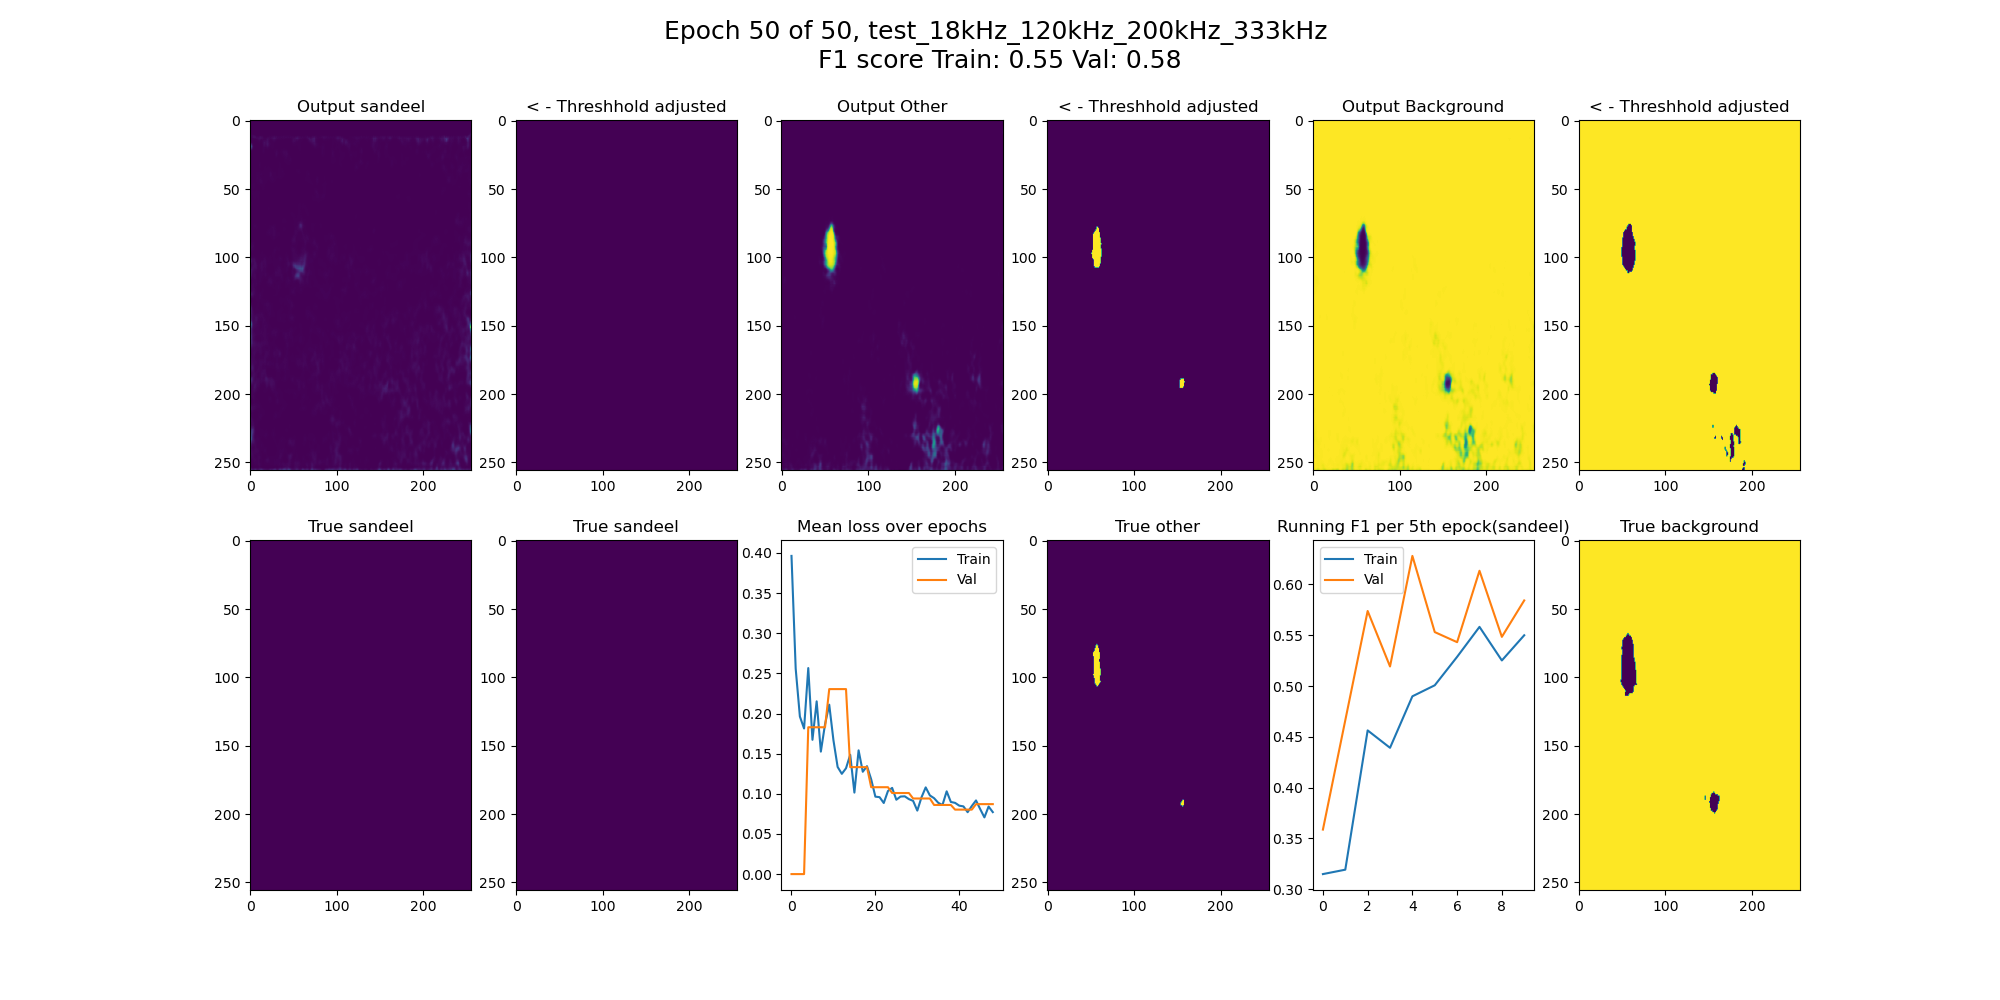
\includegraphics[scale=0.45]{figures/epoch_50_test_18kHz_120kHz_200kHz_333kHz.png}

          	\medskip 
        \end{figure}
    \clearpage
    \subsection{Subset size 5} \label{appendix:subset size 5}
        \begin{figure}[H]
             %scale=0.4,

            \hspace*{-3.2cm}
            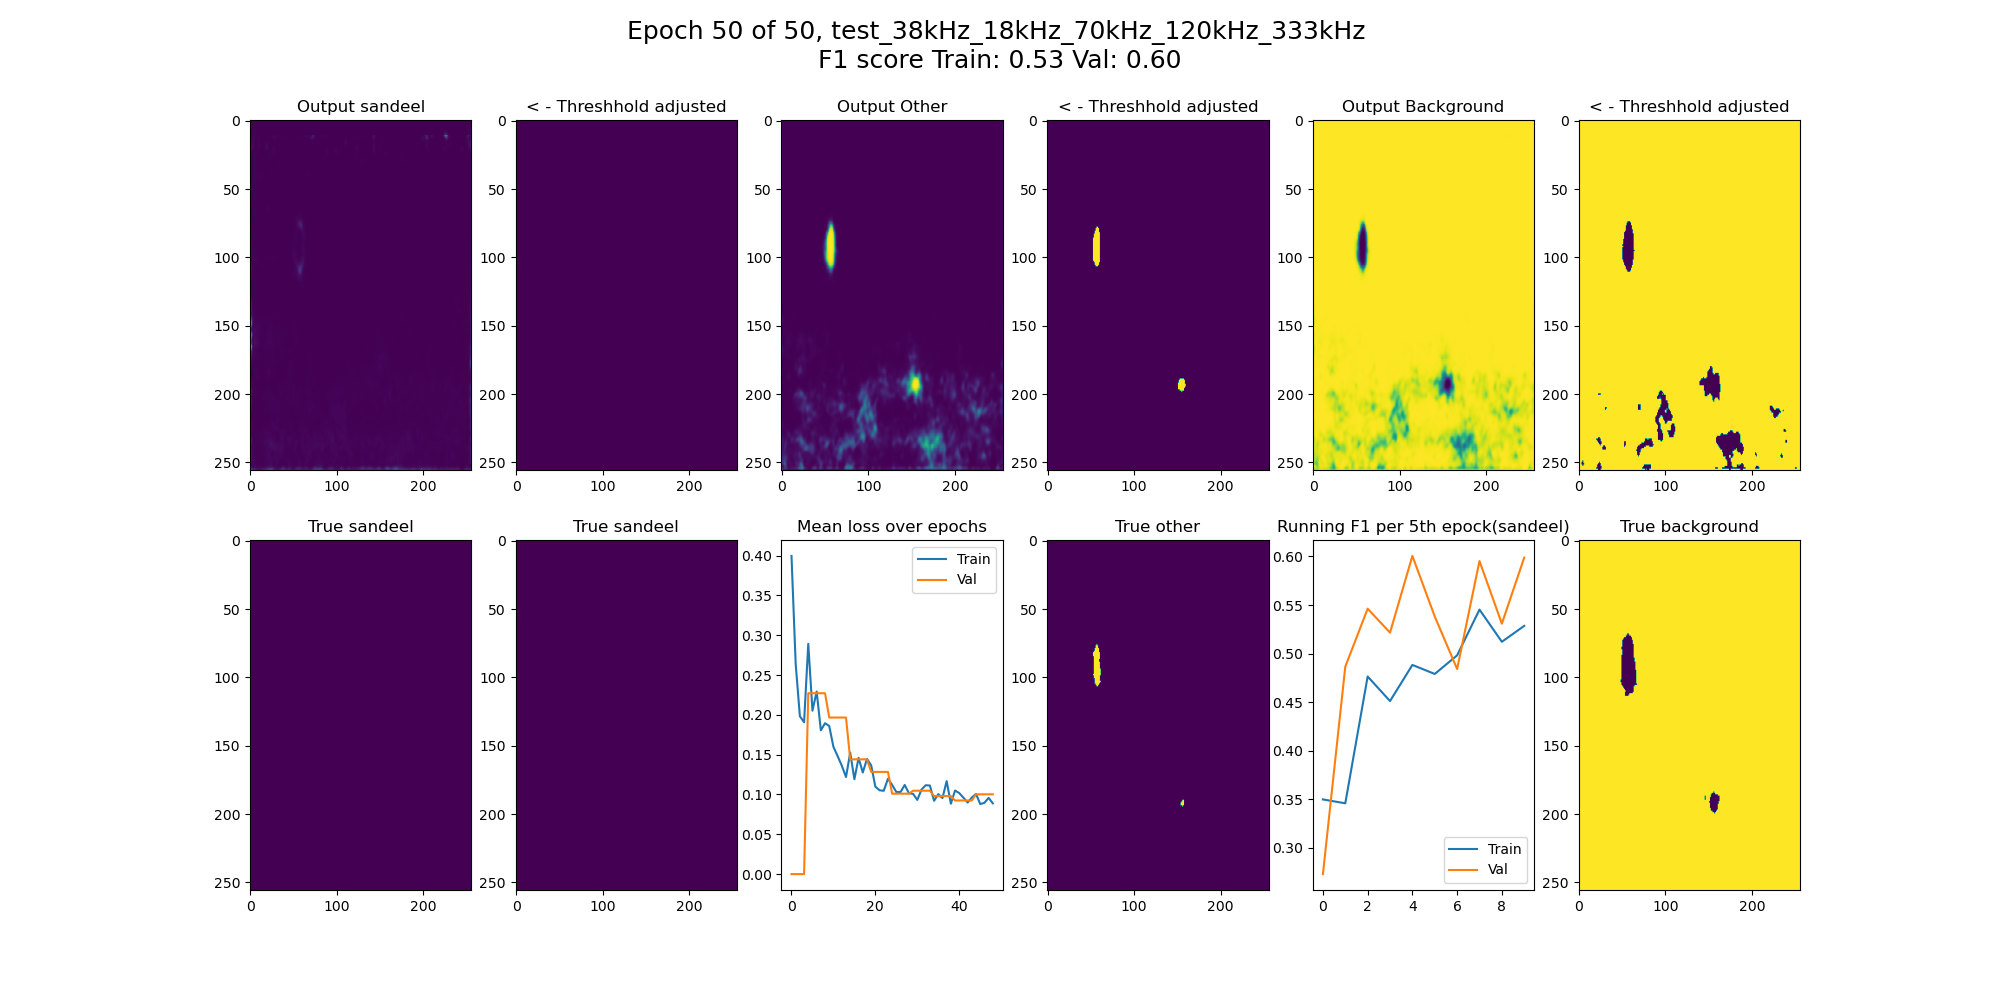
\includegraphics[scale=0.45]{figures/epoch_50_test_38kHz_18kHz_70kHz_120kHz_333kHz.png}

          	\medskip 
        \end{figure}
